% EPIC 2026 - 5th Engineering Physics International Conference
% Extended Abstract
%
% Title: Multi-Layer Swarm Quadrotor Architecture for Autonomous
%        Non-Convex Geodesic Mapping with Fault-Tolerant
%        Cooperative Coverage
%
% Template: Extended_Abstract_Template_Jun1_2026.docx
% Author Guidelines: EPIC2026_Author_Guidelines.pdf
%
% Compile: pdflatex -> pdflatex
\synctex=1
\documentclass[11pt]{article}

% ---------- Packages ----------
\usepackage[letterpaper,margin=1in,bottom=1.18in]{geometry}
\usepackage{newtxtext,newtxmath}
\usepackage{setspace}
\singlespacing
\usepackage[font=small,labelfont=bf,labelsep=quad,justification=centering]{caption}
\usepackage{tikz}
\usetikzlibrary{positioning,fit,arrows.meta,backgrounds,calc}
\usepackage{changepage}
\usepackage[numbers]{natbib}
\usepackage{enumitem}
\usepackage{hyperref}

% ---------- Formatting ----------
\pagestyle{empty}

\setlength{\parindent}{0.5em}
\setlength{\parskip}{0pt}
\setlength{\abovecaptionskip}{4pt}
\setlength{\belowcaptionskip}{2pt}

% Float parameters to prevent unnecessary page breaks
\renewcommand{\topfraction}{0.95}
\renewcommand{\bottomfraction}{0.95}
\renewcommand{\textfraction}{0.05}
\renewcommand{\floatpagefraction}{0.9}

\newcommand{\heading}[1]{%
  \vspace{1.3ex}%
  {\fontsize{10}{12}\bfseries #1}%
  \vspace{0.4ex}%
}

\newcommand{\pbody}{\fontsize{9}{11}\selectfont}

\begin{document}

% =====================================================================
% TITLE
% =====================================================================
\begin{center}
      {\fontsize{18}{22}\bfseries
            Multi-Layer Swarm Quadrotor Architecture for Autonomous Non-Convex
            Geodesic Mapping with Fault-Tolerant Cooperative Coverage
      }

      \vspace{1.5ex}

      % ---------------------------------------------------------------------
      % AUTHORS
      % ---------------------------------------------------------------------
      {\fontsize{14}{17}\selectfont
            Izma Alhazmi Herdian\textsuperscript{1,*,\textdagger},
            Sulthan Naufal Affan\textsuperscript{1,\textdagger},
            Estiyanti Ekawati\textsuperscript{1}
      }

      \vspace{1ex}

      % ---------------------------------------------------------------------
      % AFFILIATIONS
      % ---------------------------------------------------------------------
      {\fontsize{10}{12}\itshape
            \textsuperscript{1}Engineering Physics Department,\\
            Institut Teknologi Bandung, Bandung 40132, Indonesia
      }

      \vspace{0.5ex}

      % ---------------------------------------------------------------------
      % EMAIL
      % ---------------------------------------------------------------------
      {\fontsize{10}{12}\itshape
            *Corresponding author: izmaherdian@gmail.com\\
            \textdagger These authors contributed equally.
      }
\end{center}

% =====================================================================
% ABSTRACT
% =====================================================================
\vspace{1.2ex}

\begin{adjustwidth}{0.2in}{0.2in}
      \pbody
      \textbf{Abstract,} Autonomous swarm quadrotor systems have emerged as a
      promising solution for large-scale geodetic mapping in complex environments.
      This paper proposes a three-layer control architecture for resilient non-convex
      geodesic mapping using a quadrotor swarm. The high-level layer employs
      Voronoi-based non-convex region partitioning integrated with Boustrophedon
      path planning and Fault-Tolerant Cooperative Coverage (FT-CC) for adaptive
      task redistribution under failures. The mid-level layer utilizes Optimal
      Reciprocal Collision Avoidance (ORCA) for decentralized collision-free
      navigation. The low-level layer combines PID-LQR attitude control with
      PID-Hinf position control for robust trajectory tracking under external
      disturbances. The framework is validated through high-fidelity simulation
      in ROS2 Lyrical, Gazebo Harmonic, and PX4 SITL. Expected results indicate
      90--95\% coverage of non-convex regions with zero inter-robot collisions,
      demonstrating the potential of the proposed architecture for real-world
      geodetic applications.
\end{adjustwidth}

% =====================================================================
% 1. INTRODUCTION
% =====================================================================
\heading{1. INTRODUCTION}

\pbody
Swarm quadrotor systems have gained significant attention for autonomous
geodetic mapping, with applications including disaster response mapping of
post-earthquake or landslide areas, precision agriculture through
multispectral crop monitoring, environmental surveillance for forest fire
and pollution detection, and large-scale infrastructure inspection of
pipelines and bridges. In these scenarios, quadrotors equipped with optical
cameras, multispectral sensors, or radar altimeters can effectively
partition a given territory among multiple agents, enabling rapid data
acquisition over large areas through coordinated coverage. These
applications demand efficient region partitioning, robust flight control
under uncertain environmental conditions, and resilient operation despite
individual vehicle failures.

Despite progress in each domain individually, several critical gaps remain.
First, most coverage algorithms assume convex operational regions, whereas
real-world mapping areas are inherently non-convex with obstacles and
irregular boundaries. Second, end-to-end pipelines from region partitioning
to low-level rotor control are scarce, causing integration mismatches
between planning and execution layers. Third, the systematic integration of
low-level robust control, mid-level collision avoidance, and high-level
coverage planning within a unified framework has not been adequately
addressed. Fourth, fault-tolerant mechanisms in cooperative coverage for
quadrotor swarms remain underexplored, particularly under communication or
actuator failures. Fifth, validation in realistic simulation environments
with full quadrotor dynamics is still limited, with most studies relying on
simplified kinematic models. To address these gaps, this paper proposes a
three-layer architecture integrating Voronoi-based non-convex partitioning,
Boustrophedon path planning, FT-CC, ORCA-based collision avoidance, and
PID-LQR/PID-Hinf robust control, validated through high-fidelity
ROS2-Gazebo-PX4 simulation.

% =====================================================================
% 2. METHODS (OR APPROACH)
% =====================================================================
\heading{2. METHODS (OR APPROACH)}

\pbody
The proposed architecture comprises three hierarchical layers operating in a
closed loop, as illustrated in Figure~1. The high-level layer receives the
non-convex region boundary and initial drone positions as inputs. Voronoi
tessellation adapts to non-convex geometries through obstacle-aware distance
metrics, partitioning the region into sub-regions assigned to individual
drones. Boustrophedon sweeping generates optimal coverage paths for each
sub-region, minimizing overlap and energy consumption. The FT-CC module
continuously monitors drone health status and redistributes coverage
responsibilities upon detection of actuator or communication failure,
ensuring mission-level resilience. Generated waypoints are passed to the
mid-level layer.

The mid-level layer implements ORCA, a decentralized collision avoidance
protocol. Each drone broadcasts its position and velocity to neighbors,
computes velocity obstacles relative to other agents, and selects a
reciprocal collision-free velocity that preserves progress toward its
assigned waypoint. The resulting velocity commands are forwarded to the
low-level layer.

The low-level layer executes the received velocity commands through a
cascaded control architecture. PID-LQR regulates attitude angles
($\phi$, $\theta$, $\dot{\psi}$) with optimal state feedback, while
PID-Hinf provides robust outer-loop position control ($x$, $y$, $z$)
with guaranteed $H_\infty$ disturbance rejection against wind gusts and
model uncertainties. Control outputs are converted to motor PWM signals
and applied to the quadrotor plant simulated in the Gazebo Harmonic physics
engine running PX4 SITL firmware. State feedback (pose, velocity, IMU
measurements) propagates upward through all layers, enabling ORCA to
update collision avoidance decisions and FT-CC to detect faults and
trigger coverage redistribution.

% =====================================================================
% FIGURE 1 - Three-Layer Architecture
% =====================================================================
\begin{figure}[ht]
      \centering
      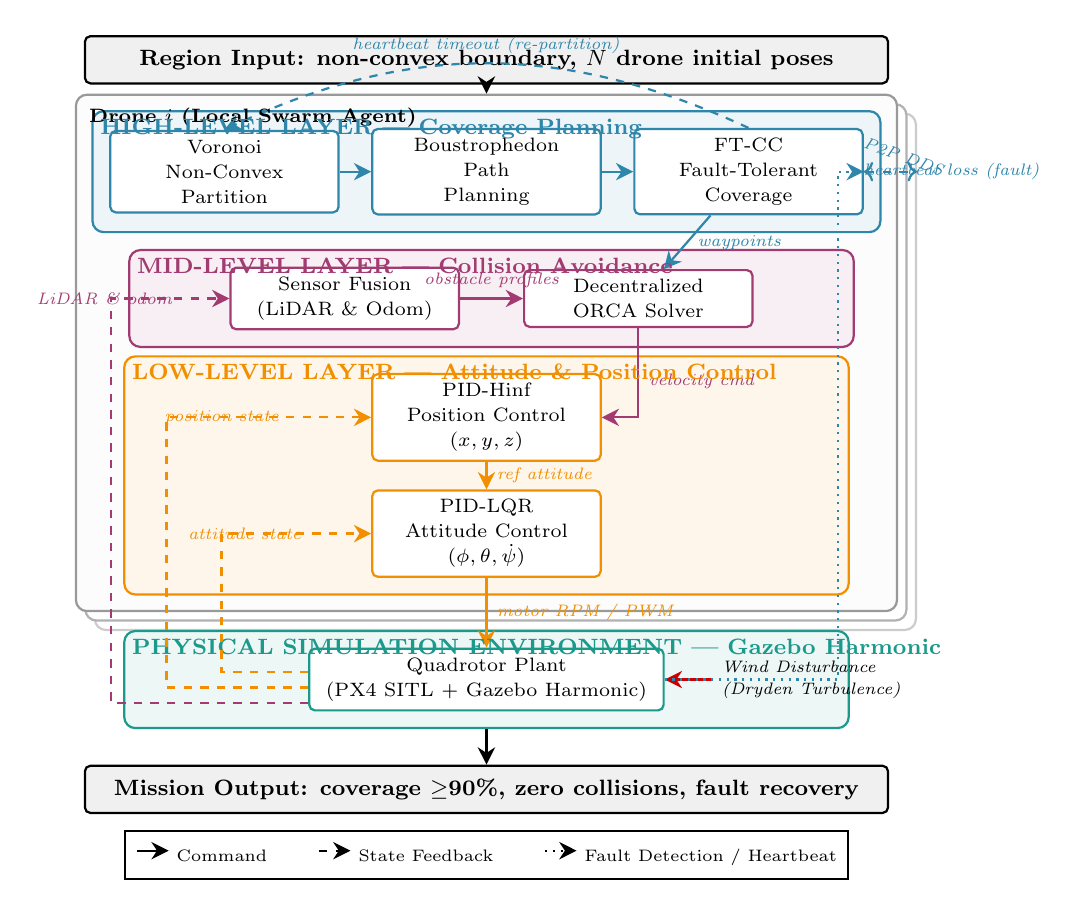
\begin{tikzpicture}[
            node distance=0.1cm and 0.4cm,
            box/.style={draw,thick,minimum width=2.9cm,minimum height=0.7cm,
                        align=center,fill=white,font=\fontsize{7.5}{9}\selectfont, rounded corners=2pt},
            layer/.style={draw,thick,rounded corners,inner sep=6pt, minimum width=9.2cm},
            arr/.style={-{Stealth[length=2.2mm,width=2.2mm]},thick},
            darr/.style={-{Stealth[length=2.2mm,width=2.2mm]},thick,dashed},
            faultarr/.style={-{Stealth[length=2.2mm,width=2.2mm]},thick,dotted},
            lbl/.style={font=\fontsize{6.5}{8}\itshape},
            ]

            % Define custom palette matching the progress report colors
            \definecolor{high}{HTML}{2E86AB}
            \definecolor{mid}{HTML}{A23B72}
            \definecolor{low}{HTML}{F18F01}
            \definecolor{sim}{HTML}{1B998B}

            % --------  INPUT BOX  --------
            \node[draw,thick,minimum width=10.2cm,minimum height=0.6cm,fill=gray!12,
                  font=\fontsize{8}{10}\bfseries, rounded corners=2pt] (input)
            {Region Input: non-convex boundary, $N$ drone initial poses};

            % --------  HIGH-LEVEL LAYER COMPONENTS  --------
            % We place Boustro in center, Voronoi left, FT-CC right
            \node[box,draw=high,below=0.55cm of input] (boustro)
            {Boustrophedon\\Path\\Planning};

            \node[box,draw=high,left=0.4cm of boustro] (voronoi)
            {Voronoi\\Non-Convex\\Partition};

            \node[box,draw=high,right=0.4cm of boustro] (ftcc)
            {FT-CC\\Fault-Tolerant\\Coverage};

            % Connect High-Level modules
            \draw[arr,high] (voronoi) -- (boustro);
            \draw[arr,high] (boustro) -- (ftcc);

            % Self-healing path-recalculation / re-partitioning loop
            \draw[darr,high,bend right=25] (ftcc.north) to node[midway,above,lbl] {heartbeat timeout (re-partition)} (voronoi.north);

            % --------  MID-LEVEL LAYER COMPONENTS  --------
            % Split ORCA block into Sensor Fusion and ORCA Solver
            \node[box,draw=mid,below=0.65cm of boustro,xshift=-1.8cm] (fusion)
            {Sensor Fusion\\(LiDAR \& Odom)};

            \node[box,draw=mid,right=0.8cm of fusion] (orca)
            {Decentralized\\ORCA Solver};

            % Connect Mid-Level modules
            \draw[arr,mid] (fusion) -- node[above,lbl] {obstacle profiles} (orca);

            % High-Level waypoints link to ORCA (as pref_vel)
            \draw[arr,high] (ftcc) -- node[right,lbl] {waypoints} (orca);

            % --------  LOW-LEVEL LAYER COMPONENTS  --------
            % Cascaded position and attitude control loops
            \node[box,draw=low,below=2.0cm of boustro] (pidhinf)
            {PID-Hinf\\Position Control\\$(x,y,z)$};

            \node[box,draw=low,below=0.35cm of pidhinf] (pidlqr)
            {PID-LQR\\Attitude Control\\$(\phi,\theta,\dot{\psi})$};

            % Connect Mid-Level command to Low-Level
            \draw[arr,mid] (orca.south) |- node[pos=0.3,right,lbl] {velocity cmd} (pidhinf.east);

            % Cascade commands
            \draw[arr,low] (pidhinf) -- node[right,lbl] {ref attitude} (pidlqr);

            % Fit the Outer Drone Swarm Containers (stacked)
            \begin{scope}[on background layer]
                  % Drone N (Backmost)
                  \node[draw=gray!40,thick,fill=white,rounded corners=4pt,fit=(voronoi) (ftcc) (pidlqr),inner sep=12pt,xshift=0.24cm,yshift=-0.24cm] (drone_n) {};
                  \node[anchor=north west,font=\fontsize{7}{8.5}\bfseries\color{gray!60},xshift=0.24cm,yshift=-0.24cm] at (drone_n.north west) {Drone $N$};

                  % Drone 2 (Middle)
                  \node[draw=gray!60,thick,fill=white,rounded corners=4pt,fit=(voronoi) (ftcc) (pidlqr),inner sep=12pt,xshift=0.12cm,yshift=-0.12cm] (drone_2) {};
                  \node[anchor=north west,font=\fontsize{7}{8.5}\bfseries\color{gray!80},xshift=0.12cm,yshift=-0.12cm] at (drone_2.north west) {Drone 2};

                  % Drone i (Frontmost)
                  \node[draw=gray!80,thick,fill=gray!2,rounded corners=4pt,fit=(voronoi) (ftcc) (pidlqr),inner sep=12pt] (drone_1) {};
            \end{scope}
            \node[anchor=north west,font=\fontsize{7.5}{9}\bfseries\color{black},inner sep=5pt] at (drone_1.north west) {Drone $i$ (Local Swarm Agent)};

            % Fit Layer Backgrounds (drawn on top of the Drone i background)
            \begin{scope}[on background layer]
                  \node[layer,fill=high!8,draw=high,fit=(voronoi) (ftcc) (boustro)] (hl) {};
                  \node[layer,fill=mid!8,draw=mid,fit=(fusion) (orca)] (ml) {};
                  \node[layer,fill=low!8,draw=low,fit=(pidhinf) (pidlqr)] (ll) {};
            \end{scope}
            \node[anchor=north west,font=\fontsize{8}{10}\bfseries\color{high},inner sep=3pt] at (hl.north west) {HIGH-LEVEL LAYER --- Coverage Planning};
            \node[anchor=north west,font=\fontsize{8}{10}\bfseries\color{mid},inner sep=3pt] at (ml.north west) {MID-LEVEL LAYER --- Collision Avoidance};
            \node[anchor=north west,font=\fontsize{8}{10}\bfseries\color{low},inner sep=3pt] at (ll.north west) {LOW-LEVEL LAYER --- Attitude \& Position Control};

            % P2P DDS Mesh network communication between High-Level layers
            \draw[darr,high,<->] (ftcc.east) -- node[above,lbl,pos=0.65,rotate=-20] {P2P DDS} (drone_n.east |- ftcc.east);

            % --------  PHYSICAL SIMULATION LAYER  --------
            \node[box,draw=sim,minimum width=4.5cm,below=0.45cm of drone_1.south] (plant)
            {Quadrotor Plant\\(PX4 SITL + Gazebo Harmonic)};

            % Command input to motor
            \draw[arr,low] (pidlqr) -- node[right,lbl] {motor RPM / PWM} (plant);

            % Wind Disturbance
            \node[lbl,right=0.6cm of plant,align=left] (wind) {Wind Disturbance\\(Dryden Turbulence)};
            \draw[-{Stealth[length=2.2mm,width=2.2mm]},thick,red!80!black] (wind.west) -- (plant.east);

            % Fit Simulation Layer Background
            \begin{scope}[on background layer]
                  \node[layer,fill=sim!8,draw=sim,fit=(plant)] (simlayer) {};
            \end{scope}
            \node[anchor=north west,font=\fontsize{8}{10}\bfseries\color{sim},inner sep=3pt]
            at (simlayer.north west) {PHYSICAL SIMULATION ENVIRONMENT --- Gazebo Harmonic};

            % --------  OUTPUT BOX  --------
            \node[draw,thick,minimum width=10.2cm,minimum height=0.6cm,fill=gray!12,
                  font=\fontsize{8}{10}\bfseries,below=0.45cm of simlayer,rounded corners=2pt] (output)
            {Mission Output: coverage $\geq$90\%, zero collisions, fault recovery};

            % Connect Input and Output
            \draw[arr] (input.south) -- (drone_1.north);
            \draw[arr] (simlayer.south) -- (output.north);

            % --------  FEEDBACK PATHS (LEFT SIDE - POSITION/ATTITUDE/SENSORS)  --------
            % 1. Attitude feedback (from plant to PID-LQR)
            \draw[darr,low] ([yshift=0.1cm]plant.west) -- ++(-1.1,0) |- node[pos=0.8,left,lbl] {attitude state} (pidlqr.west);

            % 2. Position feedback (from plant to PID-Hinf)
            \draw[darr,low] ([yshift=-0.1cm]plant.west) -- ++(-1.8,0) |- node[pos=0.8,left,lbl] {position state} (pidhinf.west);

            % 3. Sensor Feedback (LiDAR scan & neighbor odometry to Sensor Fusion)
            \draw[darr,mid] ([yshift=-0.3cm]plant.west) -- ++(-2.5,0) |- node[pos=0.8,left,lbl] {LiDAR \& odom} (fusion.west);

            % --------  FAULT DETECTION PATH (RIGHT SIDE - HEARTBEAT TO FT-CC)  --------
            \draw[faultarr,high] (plant.east) -- ++(2.2,0) |- node[pos=0.8,right,lbl] {heartbeat loss (fault)} (ftcc.east);

            % --------  LEGEND  --------
            \node[draw,thick,fill=white,font=\fontsize{6.5}{7.5}\selectfont,inner sep=4pt,
                  below=0.2cm of output.south] (legend)
            {\begin{tabular}{@{}l@{\hspace{2.5em}}l@{\hspace{2.5em}}l@{}}
                        \raisebox{0.3ex}{\tikz\draw[arr](0,0)--(0.4,0);}\ Command         &
                        \raisebox{0.3ex}{\tikz\draw[darr](0,0)--(0.4,0);}\ State Feedback &
                        \raisebox{0.3ex}{\tikz\draw[faultarr](0,0)--(0.4,0);}\ Fault Detection / Heartbeat
                  \end{tabular}};
      \end{tikzpicture}
      \caption{Proposed three-layer control architecture for resilient autonomous
            swarm quadrotor geodesic mapping.}
      \label{fig:architecture}
\end{figure}

% =====================================================================
% 3. PRELIMINARY RESULTS
% =====================================================================
\heading{3. PRELIMINARY RESULTS}

\pbody
The proposed framework is currently under evaluation through high-fidelity
simulation using ROS2 Lyrical, Gazebo Harmonic, and PX4 SITL across
multiple mission scenarios involving non-convex regions with obstacles.
Expected performance includes 90--95\% coverage completion of non-convex
regions, zero inter-robot collisions throughout the mission duration, and
successful fault recovery maintaining at least 85\% coverage after
simulated actuator or communication failure of one or more drones. The
PID-Hinf position controller is expected to outperform PID-LQR in
trajectory tracking accuracy under wind disturbance, with lower
root-mean-square error (RMSE) in hover and waypoint navigation.
Quantitative metrics including coverage ratio, collision count, trajectory
tracking RMSE, and fault recovery time will be reported in the full paper.

% =====================================================================
% 4. CONCLUSION
% =====================================================================
\heading{4. CONCLUSION}

\pbody
This paper presents a three-layer control architecture for autonomous
non-convex geodesic mapping by resilient quadrotor swarms. The main
contributions include: (i) an end-to-end pipeline integrating non-convex
Voronoi partitioning with Boustrophedon path planning and FT-CC fault
tolerance at the high level; (ii) decentralized ORCA-based collision
avoidance at the mid level; (iii) PID-LQR and PID-Hinf robust cascade
control at the low level; and (iv) validation through a high-fidelity
ROS2-Gazebo-PX4 simulation framework. The architecture addresses critical
gaps in non-convex coverage, multi-layer integration, fault tolerance, and
realistic simulation validation. Future work will focus on real-world
outdoor flight experiments and extension to heterogeneous multi-robot
teams with diverse sensor payloads.

% =====================================================================
% REFERENCES
% =====================================================================
\heading{REFERENCES}

\begin{enumerate}[leftmargin=*,labelsep=0.5em,itemsep=0pt,parsep=0pt,topsep=2pt,partopsep=0pt]
      \item {\fontsize{9}{11}\selectfont Author, A.\ et al., \emph{Journal
                  Name} \textbf{Vol}, pp.\ 1--10 (Year).}
      \item {\fontsize{9}{11}\selectfont Author, B.\ et al., in
            \emph{Conference Proceedings}, pp.\ 100--110 (Year).}
      \item {\fontsize{9}{11}\selectfont Author, C., \emph{Book Title},
            Publisher (Year).}
      \item {\fontsize{9}{11}\selectfont Author, D.\ et al., \emph{Journal
                  Name} \textbf{Vol}, Article 12345 (Year).}
\end{enumerate}

\end{document}
